\subsection{Armazenamento}

	Neste projeto será utilizada a câmera VIP E5120 IR. É uma câmera já voltada para sistemas de vigilância, muito utilizada em escritórios e shoppings.

	\begin{table}[H]
		\centering
		\begin{tabular}{|l|l|}
			\hline
			Resolução           & 1280/960       \\ \hline
			Quantidade de MP    & 1.3 MegaPixels \\ \hline
			Sensor              & Infravermelho  \\ \hline
			Alimentação         & 24Vac a 3$^a$  \\ \hline
			Compressão de vídeo & H264/MJPEG     \\ \hline
		\end{tabular}
		\caption{Especificações da VIP E5120 IR fonte: \cite{mercadoLivreVIPE5120}}
		\label{my-label}
	\end{table}

	Serão utilizadas, no total, 15 câmeras do modelo VIP E5120 IR, e para manter um armazenamento dessa quantidade vídeo, seria necessário um HD realmente potente e para tanto será utilizado o Seagate® Vídeo 3.5 HDD. Como o sistema funcionará  24x7, ou seja, 24 horas por 7 dias da semana, o servidor irá passar as imagens para o HD a uma taxa de 768 Kbps, em um mês (considerando um mês como 30 dias), será gasto um total de 3.5TB.

\begin{table}[H]
	\centering
	\begin{tabular}{|l|l|}
		\hline
		Capacidade                  & 4TB            \\ \hline
		Modelo                      & ST400DM000     \\ \hline
		Interface                   & SATA de 6 GB/s \\ \hline
		Velocidade da rotação       & 5900 RPM       \\ \hline
		Cache                       & 64 MB          \\ \hline
		Impacto máximo de operação  & 80 Gs          \\ \hline
		Tipo de armazenamento       & HDD            \\ \hline
		Comprimento                 & 147.00 mm      \\ \hline
		Largura                     & 101.85 mm      \\ \hline
		Altura                      & 26.1 mm        \\ \hline
		Peso típico                 & 610 g          \\ \hline
		AFR                         & 0.55\%         \\ \hline
		Potência média de operação  & 7.500 W        \\ \hline
		Taxa de transferência       & 600 MB/s       \\ \hline
		Taxa de dados sustentada DE & 180            \\ \hline
	\end{tabular}
	\caption{Especificações da Seagate$^{\textregistered}$ Vídeo 3.5 HDD \cite{seagate}}
	\label{my-label}
\end{table}

\begin{table}[H]
\centering
\begin{tabular}{|l|l|}
\hline
Processador              & Intel Core i7 - 4700K                                                   \\ \hline
Placa-mãe                & ASRock Z87Killer                                                        \\ \hline
Memoria                  & 16 GB G. Skill Spiner (DDR 3 - 1600/PC3 - 12800), configurada a 1600MHz \\ \hline
Placa de vídeo           & GeForce GT 630 1GB                                                      \\ \hline
Resolução de vídeo       & 1920x1080                                                               \\ \hline
Fonte de alimentação     & Corsair CX500M                                                          \\ \hline
Unidade de inicialização & Kingston HyperX 3k 480 GB                                               \\ \hline
\end{tabular}
\caption{Configuração de Hardware}
\label{tab:configHardware}
\end{table}

As câmeras serão fixadas ao balão, quando acondicionadas em seus respectivos invólucros
ou caixas de proteção. Deverão continuar operando perfeitamente sob temperatura ambiente
entre 0 e 40$^{\circ}$C e umidade relativa do ar de até 90\%.

Em tempos de muitas chuvas, ocorre uma grande variação de energia, devido às descargas
elétricas de raios. Para que não se tenha o problema de o sistema parar de funcionar por falta de
energia, e pela variação de energia, não chegar a queimar o sistema ou danificar o sistema,
será utilizado um equipamento que armazenar energia por algum tempo.

O equipamento utilizado para o sistema de energia nobreak, será o \textbf{Nobreak Organizador e
Fonte para 16 câmeras}, da tecnologia ONAT. Com este equipamento, o armazenamento de
dados terá em média 4 horas de autonomia, ou seja, caso por algum motivo a luz acabe o
sistema terá em média 4 horas funcionando perfeitamente \cite{nobreak}.

O Seagate para gravação e backup de imagens deverá ser alimentado pelo sistema de energia
(nobreak), de forma a possibilitar a operação em caso de falta de energia elétrica.

\begin{table}[H]
\centering
\begin{tabular}{|l|l|l|l|}
\hline
                      & Unidades & Preço de uma unidade & Preço total    \\ \hline
Câmera VIP E5120 IR   & 15       & R\$ 8.728,10         & R\$ 130.921,50 \\ \hline
Seagate$^{\textregistered}$ Vídeo 3.5 HDD & 4        & R\$ 984,90           & R\$ 3.939,60   \\ \hline
Sistema Nobreak       & 1        & R\$ 396,90           & R\$396,90      \\ \hline
Hardware              & 1        & R\$ 5.271,86         & R\$5.271,86    \\ \hline
\multicolumn{4}{|r|}{R\$ 140.529,86}                                     \\ \hline
\end{tabular}
\caption{Tabela de preços}
\label{table:precosComponentes}
\end{table}

\begin{figure}[H]
		\centering
		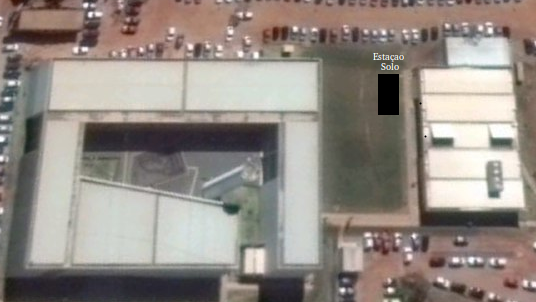
\includegraphics[width=0.6\textwidth]{figuras/estacaoSolo}
		\caption{Local da Estação Solo}
		\label{img:estacaoSoloLocal}
	\end{figure}
